\documentclass[conference]{IEEEtran}
\IEEEoverridecommandlockouts
% The preceding line is only needed to identify funding in the first footnote. If that is unneeded, please comment it out.
\usepackage{cite}
\usepackage{amsmath,amssymb,amsfonts}
\usepackage{algorithmic}
\usepackage{graphicx}
\usepackage{textcomp}
\usepackage{xcolor}
\def\BibTeX{{\rm B\kern-.05em{\sc i\kern-.025em b}\kern-.08em
    T\kern-.1667em\lower.7ex\hbox{E}\kern-.125emX}}
\usepackage{listings}
\lstset{
  frame=single,
  language=python,
  basicstyle=\small,
}

\makeatletter
\def\lst@makecaption{%
  \def\@captype{table}%
  \@makecaption
}
\makeatother

\begin{document}

\title{Benchmarking Agents Across Diverse Tasks}

\author{
\IEEEauthorblockN{Alexander Moore}
\IEEEauthorblockA{\textit{Data Science} \\
\textit{Worcester Polytechnic Institute}\\
Worcester, United States \\
ammoore@wpi.edu}

\and

\IEEEauthorblockN{Brian Lewandowski}
\IEEEauthorblockA{\textit{Computer Science} \\
\textit{Worcester Polytechnic Institute}\\
Worcester, United States \\
balewandowski@wpi.edu}

\and

\IEEEauthorblockN{Jannik Haas}
\IEEEauthorblockA{\textit{Data Science} \\
\textit{Worcester Polytechnic Institute}\\
Worcester, United States \\
jbhaas@wpi.edu}

\and

\IEEEauthorblockN{Quincy Hershey}
\IEEEauthorblockA{\textit{Data Science} \\
\textit{Worcester Polytechnic Institute}\\
Worcester, United States \\
qbhershey@wpi.edu}

\and

\IEEEauthorblockN{Scott Tang}
\IEEEauthorblockA{\textit{Data Science} \\
\textit{Worcester Polytechnic Institute}\\
Worcester, United States \\
stang3@wpi.edu}
}

\maketitle

\begin{abstract}
    Understanding which models succeed (and why) at which tasks is a foundational experience in reinforcement learning.
    Following a baseline of techniques and best practices found in the literature this project will show a comparison of multiple reinforcement learning techniques applied in a few common environments.
    In particular, this project implements several algorithms under the Q-learning, policy learning, and actor-critic categories and compares the results across several tasks.
    It is shown where these algorithms work strongly on some tasks and perform poorly on others.
    This work explores a set of baseline results for diverse reinforcement learning algorithms, in order to compare and contrast the performance of models on diverse tasks.
\end{abstract}

\begin{IEEEkeywords}
Q-Learning, Policy Learning, DQN, Policy Gradient, actor-critic, Reinforcement Learning
\end{IEEEkeywords}

\section{Introduction}
Project 3 explored how to construct a Deep Q Network (DQN) by following the classic DQN algorithm outlined originally in \cite{DQNOriginalPaper}.
Building off of this recent experience this project takes the deep learning techniques discussed in class and applies them to several well-known tasks using Q-learning, policy learning, and actor-critic methods.
The results of these methods are compared and discussed.

The openai gym \footnote{https://gym.openai.com/} was chosen to be used as the game environment.
Two games were chosen to be used for comparison of the algorithms in this paper.
First, the Breakout game was used for its familiarity from Project 3 and that it has a known level of difficulty.
In addition, it serves as a discrete action space environment.
To contrast with this, the MountainCar was also chosen as it has both a discrete and continuous action space environment available for use.
Using these environments multiple agents were trained and tested using DQN, Double DQN, Dueling DQN, REINFORCE, Proximal Policy Optimization (PPO), and Advantage Actor Critic (A2C).
This work shows that these algorithms all have strengths and weaknesses in a wide variety of areas including task completion, complexity, training time, and sensitivity to hyperparameters.

The remainder of this paper is organized as follows:
\begin{itemize}
\item Section \ref{background} provides background information regarding the methods implemented.
\item Section \ref{methodology} provides a description of the methodology used to train, execute, and assess the algorithms explored.
\item Section \ref{results} provides a discussion of the training process and associated results.
\item Finally, the paper concludes in section \ref{conclusion}.
\end{itemize}

\section{Background Information} \label{background}

\subsection{Deep Q Learning}
Deep Q learning uses a deep neural network to learn coefficients $\omega$ such that the network's value function evaluates $(state, action)$ pairs improving the model's task reward. For some of our environments this will be a convolution over a screen space, and for some we might extract some derived features about the game for the model to use as a state representation.

\subsection{Double Deep Q Learning}
Double deep Q networks address the maximization bias problem from Deep q learning by instead letting two Q functions randomly select the action and update the corresponding Q function. This process inhibits bias and will potentially converge faster or outright outperform DQN on all tasks.

\subsection{Dueling Deep Q Learning}
Dueling DQN separates the Q-learning process into two functions, the sum of the state and state-action estimator models. This approach ideally learns how to relatively value states by accounting for a learned state-value function $V(s)$, as well as an advantage function $A(s,a)$ interpreted as the value of taking action $a$ while in state $s$. For this reason this different approach will be interesting to analyze on tasks where the actions might not always directly affect the environment, for example in breakout where many movements have no direct affect on the game environment.

\subsection{Basic Policy Gradient}
Policy gradient algorithms in general are methods that learn a parameterized policy that can select actions without consulting a value function \cite{ReinforcementLearningBook}.
A value function may be utilized or learned to support learning a given policy, however, it is not involved in the process of choosing an action with these methods \cite{ReinforcementLearningBook}.
The Basic Policy Gradient algorithm treats learning of the policy as an episodic case using a performance measure that equates to the reward obtained following the current policy given a starting state of an episode. 
At its core, the Basic Policy Gradient algorithm takes the gradient of expected rewards for an episode and uses it to update the policy parameters.
This can be summarized by the two equations below,

$$\nabla \bar{R}_{\theta} = \frac{1}{N} \sum \limits_{n=1}^N \sum \limits_{t=1}^{T_n} R(\tau^n) \nabla log\pi_{\theta}(a_{t}^n | s_{t}^n)$$

$$\theta = \theta  + \eta \nabla \bar{R}_{\theta}$$

where N is the number of episodes, T is the steps within an episode, R is the reward for a given episode, $\theta$ are the policy parameters, a is a given action, and s is a given state.

Implemented in pseudocode, this algorithm would be similar to Listing \ref{listing:basicPolicyGradientAlg}.
While not implemented as part of this project is is the building block for all subsequently developed policy gradient models.

\begin{lstlisting}[
    float=t,
    caption=\textbf{Basic Policy Gradient} The basic policy gradient algorithm,
    label=listing:basicPolicyGradientAlg,
]

Loop until stopping criteria met:
    for a batch of episodes:
        - Step through episode
        - Store reward gained

    - Determine reward gradient of batch
    - Update policy parameters
\end{lstlisting}

\subsection{REINFORCE Policy Gradient}
The REINFORCE Policy Gradient method also referred to as Monte-Carlo Policy Gradient makes a slight adjustment to the Basic Policy Gradient algorithm of using the return from each time step instead of the overall reward from the episode in the update of the policy parameters. This will reduce the high variance of the standard basic policy gradient algorithm.
This change can be seen in the pseudocode in Listing \ref{listing:reinforcePolicyGradientAlg}. 

\begin{lstlisting}[
    float=h,
    mathescape = true
    caption=\textbf{REINFORCE Policy Gradient} The reinforce policy gradient algorithm,
    label=listing:reinforcePolicyGradientAlg,
]

For each episode from the current policy:
    For t=1 to T-1 do:
        {$\theta = \theta  + \alpha \nabla_{\theta} log\pi_{\theta}(s_t, a_t)G_t$}

    end for
end for
return {$\theta$}
\end{lstlisting}

\subsection{PPO Policy Gradient}
Unlike the Basic and REINFORCE policy gradient algorithms, the Proximal Policy Optimization (PPO) algorithm is an off-policy method, where the performance assessment and improvement of a policy is different than the one used for action selection (or sampling). The separate policies allow the collected data to be used more than once, which result in faster performance. PPO also addresses other shortcomings of the Basic Policy Gradient by subtracting the state-value off as the baseline to improve update accuracy when rewards are non-negative via an Advantage function. This function also serves to reduce large variance without increasing bias. Finally, PPO improves stability by imposing a constraint on the distance (or difference) between the old and new policies by clipping their ratio to a small interval around one.

\subsection{Advantage Actor Critic}
Actor-Critic methods, similar to the REINFORCE algorithm, learn both a policy function and state-value function.
The main difference between them, however, is the fact that actor-critic methods use the value function as a way to bootstrap the value estimation.
The implementation for this work follows closely to the "One-step Actor-Critic" algorithm outlined in \cite{ReinforcementLearningBook} with some practical updates for implementation.
It is a temporal difference algorithm that relies solely on the current step for learning.
This is in contrast to the many of the other algorithms implemented in this work as they involve utilizing a replay buffer for batch learning.

In addition, it should be noted that this implementation remains a basic implementation and does not include the commonly seen updates added to this method such as an additional entropy loss.

\section{Methodology} \label{methodology}

\subsection{Tools and Environment}
This project was implemented using the Python language and relied heavily on the openai gym packages.
In addition, the code from Project 3 was adapted to serve as a baseline for interacting with the gym environments described next.

\subsubsection{BreakoutNoFrameskip-v4}
The Breakout environment involves interacting with the Atari 2600 game by the agent receiving image data for what has been seen on screen.
After pre-processing handled by the atari wrapper code the state space consists of 4 stacked 84x84 images.
The action space for this environment consists of 4 possible discrete actions:

\begin{itemize}
    \item LEFT - Move agent left
    \item RIGHT - Move agent right
    \item NOOP - Do nothing
    \item FIRE - Places ball in motion at start of new lives
\end{itemize}

This environment was chosen as it was familiar from Project 3 and sufficiently difficult for naive models.
In addition, it serves as a well-contained discrete action space for all algorithms under test.

The reward structure for this environment consists of the traditional values for the blocks in the game where the first two levels provide one point, the next two levels provide 3 points, and the final two levels provide 7 points.
For the learning agent, the atari wrapper environment clips this reward to be just one point for a timestep where a brick was broken.

\subsubsection{MountainCarContinuous-v0}
The Mountain Car environment in both its original and continuous form consists of the agent being a car beginning in the valley between two mountains.
In this classic control task, the agent must apply a specific force to the mountain car with the goal of reaching the top of the right hand mountain as seen by the flag in Figure \ref{fig:mountainCarEnvironment}.

\begin{figure}[htbp]
\centerline{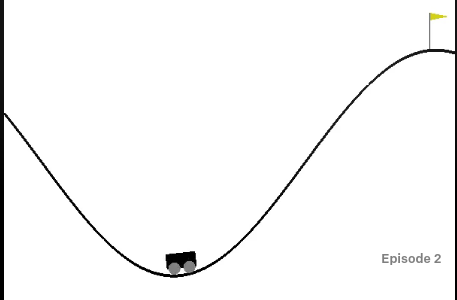
\includegraphics[scale=0.5]{mountain_car.png}}
\caption{\textbf{Example of the Mountain Car Environment}  The mountain car environment provided by openai.}
\label{fig:mountainCarEnvironment}
\end{figure}

In this environment, the agent must learn to gather enough momentum by first going backwards a bit prior to going forwards in order to have enough acceleration to reach the flag.

The state space for this environment consists only of the mountain car's position and velocity.
The action space for this environment is a single continuous action which is the force to be applied to the mountain car.
A positive value is a force towards the goal and a negative value for this force puts the mountain car in reverse.

The reward structure for this environment consists of the agent receiving a small negative reward for the number of actions taken and a positive reward of 100 when reaching the goal.
This environment is considered solved once a score of 90 is achieved \footnote{https://github.com/openai/gym/wiki/MountainCarContinuous-v0}.

This environment was chosen as it is a well-suited introductory environment to explore continuous action spaces.

\subsubsection{MountainCar-v0}
The MountainCar-v0 environment is the discrete action-space relative of MountainCarContinuous-v0 as described above.
This environment entails the same general principles and overall goal but the action space has been altered to use discrete actions as listed below.

\begin{itemize}
    \item PUSH LEFT
    \item PUSH RIGHT
    \item NO PUSH
\end{itemize}

The state-space for this environment remains unchanged.
The reward structure for this environment consists of -1 for each time step until the goal is reached.
The environment is considered solved if an average of -110 points is achieved over 100 consecutive trials \footnote{https://github.com/openai/gym/wiki/MountainCar-v0}.

\subsection{Continuous Action Spaces}

\section{Results} \label{results}

\section{Planned Work} \label{planned}

\subsection{Background Research}
Research is planned to be performed to understand all of the techniques to be exercised during this project.
In addition, the literature will be surveyed to identify any recent developments or improvements related to the methods being employed.
While doing this, we also plan to obtain available benchmarks for techniques such as those found in \cite{DQNOriginalPaper, NatureDeepLearning, bhonker2017playing}.
To keep experiments fair to models and reduce compute time, we will find hyperparameter suggestions by model authors where available, but not directly tune one model's hyperparameters for a single game task. Rather, heuristics will be used in their place to attempt to simultaneously generalize models across tasks while keeping experimental design relatively fair.

\subsection{Environment Setup}
This part of the project involves ensuring that all team members have the ability to develop and assess the algorithms under study.
Some of the key areas include ensuring a common (or compatible) software environment is available including the ability to run \cite{nichol2018retro} either locally or on a WPI asset such as the Ace cluster.
In addition, a simple framework or skeleton code should be utilized such that all algorithm implementations are structurally similar.
We plan to take advantage of the provided framework from Project 3 to reduce the amount of work necessary in this area.

\subsection{Algorithm Implementations}
The algorithm implementations involve taking the actual theoretical algorithms and implementing them in Python code using common libraries such as PyTorch and NumPy.
The goal of these implementations is to be true to the algorithms and any notable improvements that have become common in practice.
While deviations and modifications to these algorithms may become necessary for practical reasons, they will be noted in the final report provided, and no modifications would be made which fundamentally alters the behavior of agents in the games we are testing. The primary goal is to evaluate convergence speed, time to a goal score, and consistency of results across tasks.

\subsection{Results Analysis}
During the analysis of the results each model will be compared using common metrics such reward per episode and the number of episodes necessary for convergence.
In addition, commentary will be provided of any interesting results or findings from the experiments that do not fit into the objective metrics being measured.
We will incorporate our knowledge from researching capabilities of the models as well as our intuitions gained from implementing the algorithms to analyze their performances in both testing and training. After considering case-by-case performances of each model, we can consider the field of agents to determine if there is a subset of 'best' models which consistently outperformed their peers, and maintained that success even across diverse tasks. Ranking quality of models across these tasks can be done with metrics such as training time to achieve a threshold score, max score reached given a limited training time, and consistency of performance across tasks.

\subsection{Work Completed}

Our largest contribution to the final deliverable so far is the development of an agent-game pair running file, in which the researcher inputs arguments into the terminal corresponding to the model and task they would like to dispatch for training. This means all of our model implementations must be written such that they are indifferent to different environment types, state shapes, model attributes, or other quirks arising in agent training. This means that all agents must inherit from a superclass of a general agent framework, and particularities in training (such as the difference between training on state-action-reward tuples, episodes, or tuples of episodes must be addressed in one execution of the model's unique 'train()' function, which is called in the general 'agent\_runner' executed file.
At the testing time determined by the 'agent\_runner' call, this same process occurs though in a simpler fashion where the generic 'agent.make\_action' refers to a trained policy and state-value function to play the game it was trained on.
The development of this general dispatcher will serve two primary purposes for the remaining work of the project. First, this shared dispatcher file will assure consistent running of each model, where changes can be made to environments and shared parameters without needing to rely on manual changes to many ($num\_tasks*num\_agents$) files. Second, this greatly expedites batch computation when training models on cluster computers, as we can serialize calls for any number of agents, games, and hyperparameters as we see necessary.

So far, we have draft versions of the following algorithms:
\begin{enumerate}
\item Policy Gradient REINFORCE
\item DQN
\item Double DQN
\item Dueling DQN
\end{enumerate}

The following algorithms are unstarted or in a very early stage:
\begin{enumerate}
\item PPO Policy Gradient
\item Basic Policy Gradient
\end{enumerate}

\subsection{Paper Preparation}
A roughly 10 page paper will be put together to conclude this project and communicate its findings.
This paper will include any background information necessary for the project, a description of algorithms used and considered, implementation methods, results, and analysis.

\subsection{Presentation Preparation}
The work of this project will be summarized in a presentation to be delivered on the poster day for the project.
If any work is found to be an interesting demo it would be displayed during the presentation time. Potential presentation results include:
\begin{itemize}
    \item Expected score in testing after a fixed training time in seconds or iterations for each game
    \item Necessary training time in seconds or iterations to achieve a fixed score for each game
    \item Comparison of learning rates of models for each game
    \item Meta-comparison of games, their action spaces, and relevant challenges and tasks. This will include discussion on the nature of each algorithm as well as our expectations for the performance given the quirks of each task. We will include mathematical intuition for why some models would struggle or fail to learn in some environments.
\end{itemize}

\section{Tools and Environment}

\subsection{Implementation Language}
This project will be using the Python language of at least version 3.7.
In addition to the standard libraries, it is expected that the following additional libraries will be utilized and standardized across group development machines:
 
\begin{itemize}
    \item Gym Retro \cite{nichol2018retro}
    \item PyTorch
    \item NumPy
    \item Matplotlib
    \item Pandas
\end{itemize}

In addition, the framework from Project 3 will be utilized as a baseline for implementing the various algorithms being researched. Each algorithm can be fit in this framework to facilitate plug-and-train pipelines for each different model and game.

\subsection{Reinforcement Learning Environment}
This project plans to use an existing reinforcement learning environment while assessing the various algorithm implementations.
In particular, the Retro Learning Environment \cite{nichol2018retro} will be utilized for its large selection of games with high levels of complexity.
We maintain the usage of the Atari Breakout gym environment for multiple reasons. The breakout environment will be familiar to our peers as something they worked extensively with on project 3, and know the implementation tricks as well as the expected rewards of a DQN model, for example. This will contextualize a results plot which shows perhaps that DQN is outperformed by other models, to some comprehensible scale.
In addition, it maintains the same API as the environment used in Project 3 making it close to a drop-in replacement for the existing Project 3 framework with our mentioned extensions to add robustness to model differences, game flexibility, and other algorithm needs.

The initial plan was to focus on the games explored in \cite{bhonker2017playing} as there is a baseline result for several algorithms and a known level of complexity.
Some of the options to be explored include F-Zero, Gradius 3, Mortal Kombat, and Wolfenstein.
We have altered this course to instead use a simple by continuous-space environment provided by the OpenAI Gym. This will lead to stability in comparing the tasks, as the environments are provided by the same source despite the games being very different. In addition a simpler task might lead to more reasonable results, where we know even DQN can have some small success, where we worried that extremely complex games might lead to uninteresting results if some models fail to learn any meaningful parameters during training.
Note that the choice of game is subject to change depending on availability of published results and practical reasons given the time frame for the project.
These games represent diversity in action spaces, reward sparsity, action-memory importance, and state dimensionality.

\subsection{Compute Resources}
The plan for compute resources is to use a combination of local machines as well as the Ace cluster at WPI.
Several team members have access to personal machines with GPUs while other team members have access to the Ace cluster.
These resources combined should provide sufficient computing resources to be successful on this project.
Dispatching batches of jobs can also expedite and parallelize long training times. Compute resources were a limiting factor for the developement of this project, as each of the agent-model-task combinations must be trained independently and for each combination of hyperparameters. Since project 3 took many weeks to optimize just a single agent-task combination with some parameter set, optimizing up to 12 experiments would be intractable, as though there is some carryover between parameter choices between similar agents on the same task, these parameters do not carry over between tasks, and there is a massive space of parameters to explore, particularly when agents include their own unique parameter options. The implementation of such arguments alone is a large task to handle over multiple tasks.

\section{Final Deliverables} \label{deliverables}

\subsection{Final Report}
The final report provided as part of this project will include the necessary background information required to understand the methods used.
In addition, our findings on $N*K$ trained models where N is our number of agents and K is our number of games will be included.
The analysis of our findings will include theory on why some models performed better or worse given the game tasks, appropriate model choices for different tasks, and a discussion on our findings of what succeeded and failed for developing diverse models over diverse tasks.
In addition, a description of our methodology will be provided such that others could use our workflow to do the same experiments.

\subsection{Poster Presentation}
The presentation delivered as part of this project will provide an overview of the information covered in the final report.
This includes brief background information and a focus on the comparative results received.
If applicable, any live demos will be rendered and performed during this portion of the project. These live demos will include some subset of our experiments, likely our best-trained models on the Breakout and MountainCar tasks rendered by the built-in functionality of the Atari and Box2d environments.

\subsection{Code and Model Artifacts}
All code and artifacts needed to duplicate this project will be provided as part of the deliverables for this project.
In addition, all trained models used in reported performance measures will be saved and provided.

\section{Conclusion} \label{conclusion}
Here, there should be an in-depth discussion about the way each model performed on each task and how those findings either agree or disagree with our expectations and hypotheses about the models, tasks, agents, and parameters.

This project represents an approximate survey of diverse models from the Reinforcement Learning course, as well as the challenges and benefits of implementation of these methods on very different tasks. The project goal was effectively a combination of 6 models across 2 tasks, taking for 12 applications of a Project-3-like assignment. However, instead of simply doing 12 unique projects, this group wanted to emphasize the contrast in application between these different models on these different tasks.

Among the time-expensive nature of training many agents on multiple tasks, our largest efforts were in the developement of so many different models. These difficulties were effectively 6-8 project three developement times, as we split the agent developement among team members. In hindsight, in order to better address the goals of this project, we would make some changes to the experimental design and workflow of the project. Having a shared `agent_runner` was a huge benefit, but instead of using that common core to develop many diverse agents, it is possible we could better address the goals of the experiment by using fewer models and more tasks. This change would give a better sense of the __benchmarking__ goal, as it would be interesting to compare some kind of human-performance normalized results of a handful of agents (DQN, policy gradient,) on many tasks, such as every atari game. As it stands, the deployment of more agents is an interesting comparison on a small number of tasks, but most of our resources went into the developement of these diverse agents, as opposed to truly optimizing and benchmarking them. Another option to ameliorate these difficulties would be to rely only on other researcher's implementations of these algorithms, so that our group could focus on applying them and getting as many results as possible, instead of troubleshooting and programming.

\bibliography{citations.bib}{}
\bibliographystyle{plain}

\vspace{12pt}

\end{document}
